\documentclass[border=10pt,tikz]{standalone}
\usepackage{tikz}
\usetikzlibrary{positioning,arrows.meta,shapes}
\begin{document}
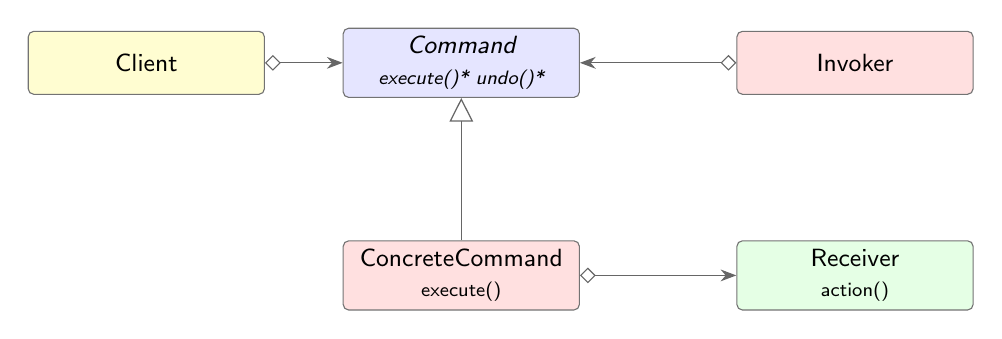
\begin{tikzpicture}[
  font=\sffamily\small,
  cls/.style={rectangle, rounded corners=2pt, draw=black!55, line width=0.4pt,
              minimum height=8mm, minimum width=30mm, inner sep=3pt, fill=white, align=center},
  abs/.style={cls, fill=blue!10, font=\sffamily\itshape\small},
  con/.style={cls, fill=red!12},
  imp/.style={cls, fill=green!10},
  cli/.style={cls, fill=yellow!18},
  inh/.style={-{Triangle[length=3mm,width=3mm,open]}, draw=black!60, line width=0.45pt},
  agg/.style={{Diamond[length=2mm,width=2mm,open]}-{Stealth[length=2mm]}, draw=black!60}
]
\node[cli] (c)   at (-5, 1.5) {Client};
\node[abs] (cmd) at (-1, 1.5) {Command \\ \scriptsize execute()*  undo()*};
\node[con] (cc)  at (-1,-1.2) {ConcreteCommand \\ \scriptsize execute()};
\node[imp] (rcv) at ( 4,-1.2) {Receiver \\ \scriptsize action()};
\node[con] (inv) at ( 4, 1.5) {Invoker};

\draw[agg] (c.east) -- (cmd.west);
\draw[inh] (cc.north) -- (cmd.south);
\draw[agg] (cc.east) -- (rcv.west);
\draw[agg] (inv.west) -- (cmd.east);
\end{tikzpicture}
\end{document}
